% Chapter 3
\chapter{Estado del Arte}
\label{Chapter3} % Change X to a consecutive number; for referencing this chapter elsewhere, use \ref{ChapterX}

En este Capítulo se encuentra el estudio de los trabajos anteriormente realizados que están relacionados con nuestro proyecto terminal, esto con la finalidad de presentar antecedentes, y dejar ver discrepancias y similitudes con el nuestro.\newline

El trabajo de dimensionar los sistemas de comunicación móviles es una necesitad recurrente en cada generación, En \parencite{Celis2016}, se encuentra un proyecto terminal realizado por alumnos de la UPIITA, en el cual se realizó una simulación, bajo el paradigma de eventos discretos, de un sistema celular 4G, con un enfoque en distintos esquemas de reúso de frecuencias y calendarizadores para obtener resultados sobre qué combinación de estos y bajo qué condiciones permitían al sistema tener un mayor desempeño. En este proyecto la simulación se llevó a cabo utilizando Matlab, el paradigma de programación fue el de eventos discretos por lo que presenta un buen precedente a nuestro proyecto.\newline

Por otra parte, el reciente crecimiento de los casos de uso de IoT en una amplia gama de aplicaciones industriales, de servicios públicos y ambientales ha exigido la necesidad de la caracterización del tráfico tipo máquina (MTC). Reconociendo la importancia de este tráfico, la 3GPP ha propuesto dos modelos de tráfico, que modelan el tráfico agregado generado por una gran cantidad de dispositivos. El primero modela el tráfico generado aleatorio, mientras que el segundo modela el tráfico síncrono con el tiempo. Dado que los modelos solo se centran en el tráfico agregado, no son apropiados para el análisis práctico porque no son lo suficientemente precisos como para representar un tráfico M2M real y los modelos no permiten la manipulación máquina por máquina lo que hace difícil para integrar el tráfico en redes celulares.\newline

En \parencite{Gupta2018}, los autores consideraron modelar el tráfico de dispositivos IoT conectados a través de tecnologías LPWAN. Debido a las diversas aplicaciones de IoT, no es trivial tener un solo modelo de tráfico para representarlos a todos, el tráfico puede clasificarse ampliamente como periódico, desencadenado por eventos o una combinación de ambos. Evaluaron el rendimiento de LoRaWAN, en presencia de un híbrido de ambos tipos de tráfico, donde el evento se propaga espacialmente a lo largo del tiempo. Utilizaron el modelo CMMPP para representar dicho tráfico característico de dispositivos IoT independientes activados por un evento. Ya que en una implementación práctica de dispositivos IoT basados en sensores, estos generalmente se implementan densamente para garantizar una medición suficiente y confiable. De este modo, cuando ocurre un evento, exhiben correlación espacial y temporal en su velocidad de tráfico debido a los fenómenos naturales de la métrica que miden. \newline

De igual manera pero ahora con un enfoque en sistemas celulares LTE, en \parencite{Smiljkovic2014} los autores analizaron el tráfico M2M con velocidad de datos variable bajo el supuesto de que la red LTE tiene recursos limitados. Los resultados muestran las características del tráfico M2M de una manera más realista, identificando las diferencias del tráfico estándar en la red celular. Revelan que el tráfico cuenta con la propiedad de auto similitud solo para una gran cantidad de MTC. Además, los resultados dan una idea de los parámetros de diseño que deben considerarse para LTE a fin de admitir el tráfico M2M.\newline

Estos trabajos son una gran aportación ya que demostraron que se puede usar un modelo de tráfico CMMPP para evaluar el impacto en la tecnología de radio IoT, configurando adecuadamente el modelo para representar casos de uso del mundo real. La integración del tráfico M2M en las redes celulares existentes será parte inevitable de la evolución de las redes. En nuestro proyecto se planea evaluar este modelo CMMPP, pero enfocado en sistemas celulares 5G donde se esté dando servicio a usuarios NB-IoT de distintas aplicaciones, además, consideramos un esquema de acceso al medio para la compartición eficiente de los recursos.\newline

Ahora bien, del lado de los esquemas de acceso no ortogonales (NOMA) en redes de quinta generación, y más en concreto de NOMA bajo estándares de 5G/IoT, se ha trabajado arduamente ya que el tema de maximizar la conectividad de los sistemas en escenarios masivos de usuarios esperados en sistemas 5G/IoT son una gran discusión de interés en la actualidad. Dentro de la literatura científica se encuentra toda una gama de propuestas de diferentes modelos de sistema relacionados a NOMA.\newline

En \parencite{Zhang2017}, los autores proponen un sistema usando geometría estocástica (PPP) para modelar un ambiente inalámbrico denso que admita NOMA tanto en el enlace de subida como en el enlace de bajada; el modelado es analítico y validado por simulación. \newline

En la implementación de NOMA proponen dos esquemas de emparejamiento de usuario: uno aleatorio y otro selectivo:
\begin{enumerate}
\item  Cuando el agrupamiento es aleatorio, los UE son seleccionados aleatoriamente.
\item  Cuando el agrupamiento es selectivo, el primer UE deberá tener una relación señal-interferencia más ruido (SINR) por encima del umbral T1 y el segundo UE tiene un SINR por debajo del umbral T2, T2 $\mathrm{\le}$ T1.
\end{enumerate}

Consideraron un error de propagación SIC durante el proceso de decodificación por parte del UE. Además, optaron por una estrategia de asignación de potencia fija, donde la potencia de enlace de bajada asignada a un UE está predefinida y permanece sin cambios.\newline

\begin{figure}
\centering
\begin{minipage}{.45\linewidth}
  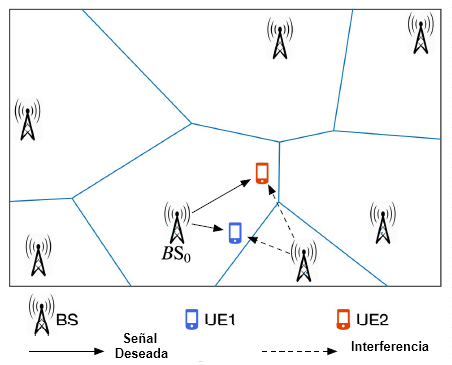
\includegraphics[width=\linewidth]{Modelo de sistema para el sistema de enlace descendente NOMA}
  \captionof{figure}{Modelo de sistema para el sistema de enlace descendente NOMA}
  \label{fig:img1}
\end{minipage}
\hspace{.05\linewidth}
\begin{minipage}{.45\linewidth}
  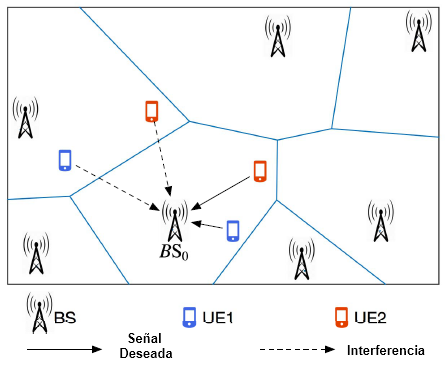
\includegraphics[width=\linewidth]{Modelo de sistema para el sistema de enlace ascendente NOMA}
  \captionof{figure}{Modelo de sistema para el sistema de enlace ascendente NOMA}
  \label{fig:img2}
\end{minipage}
\end{figure}

Las ganancias implementan el desvanecimiento de Rayleigh entre la $BS_0$ y $UE_i$. La ganancia en potencia de desvanecimiento Rayleigh entre BS y UE sigue una distribución exponencial con media 1 y se distribuye de forma independiente e idéntica (i.i.d.)\newline

En el enlace descendente (DL), se agregaron perdidas por trayectoria con un exponente de pérdida y se calcula la interferencia entre celdas cumulativa de todas las bases adyacentes. En el enlace ascendente (UL), la interferencia inter-celdas proviene de todos los otros UEs que comparten la misma sub-banda. \textit{[Véanse Figuras~\ref{fig:img1}, \ref{fig:img2}]}\newline

Como se puede observar, este trabajo se enfocó en NOMA pero para sistemas 5G en general, sin embargo no consideraron la actuación de dispositivos IoT los cuales al tener diferentes calidades de servicio, impactaría en la toma de decisiones con respecto a NOMA, más en concreto en el emparejamiento de usuarios.\newline

Por el contrario, un grupo de autores de la Universidad Británica de Columbia\parencite{Mostafa2019} han trabajado en emplear NOMA para mejorar la densidad de conexión en los sistemas NB-IoT. En su propuesta cada subportadora puede dar servicio máximo a dos dispositivos con diversos requisitos de QoS. \newline

Formularon problemas de asignación de potencia de transmisión y subportadora conjunta para los modos singletone y multitone.  Además, propusieron algoritmos heurísticos con baja complejidad y dieron como resultado un rendimiento cercano a las soluciones óptimas y subóptimas en ambos casos. Los resultados de la simulación mostraron que el uso de NOMA aumentó la densidad de conexión hasta en un 87\% en comparación con OMA en el modo singletone y en el modo multitono, la densidad de conexión también se incrementó hasta en un 24\%.\newline

Los autores en \parencite{Shahini2019} desarrollaron un esquema NOMA en el dominio de potencia con agrupación de usuarios en un sistema NB-IoT. Resolvieron un problema de optimización para maximizar el rendimiento total de la red al optimizar la asignación de recursos de los dispositivos MTC y la agrupación de NOMA al tiempo que satisface los requisitos de potencia de transmisión y QoS. Además, diseñaron un algoritmo heurístico eficiente para resolver el problema de optimización propuesto mediante la optimización conjunta de la agrupación NOMA y la asignación de recursos de dispositivos MTC.\newline

En su modelo de sistema consideraron un escenario de una única celda (solo un eNB), que admite dispositivos MTC basado en el estándar NB-IoT. Asumieron que no hay interferencia entre células de otras células vecinas. \newline

\begin{figure}[th]
\centering
\includegraphics[scale=.6]{Figures/Modelo de sistema de una sola celda usando clusterización}
\decoRule
\caption[Grupos NOMA que incluyen dispositivos mMTC y URLLC, donde los dispositivos MTC comparten los subcanales asignados a cada clúster NOMA.]{Grupos NOMA que incluyen dispositivos mMTC y URLLC, donde los dispositivos MTC comparten los subcanales asignados a cada clúster NOMA.}
\label{fig:NOMA_NBIOT}
\end{figure}

Propusieron un esquema NOMA de dominio de potencia agrupando (de entre 1 a 4) dispositivos mMTC y URLLC en una red NB-IoT como se muestra en la Figura~\ref{fig:NOMA_NBIOT} . Según el esquema NOMA, los dispositivos mMTC y URLLC comparten cada subportadora (subcanal) y transmiten datos de manera no ortogonal, es decir, más de un usuario puede compartir el mismo subcanal. Por lo tanto, los dispositivos se dividen en diferentes grupos, llamados grupos NOMA. Para decodificar con éxito los mensajes del mensaje recibido combinado, el eNB emplea el esquema SIC. Por lo tanto, los usuarios deben ordenarse en cada grupo de acuerdo con el método SIC.\newline

Como vemos, se ha investigado bastante acerca del desempeño de los esquemas NOMA para IoT, sin embargo nuestra propuesta resulta diferente ya que además de considerar un escenario celular bajo un esquema PD-NOMA, se propone implementar un despliegue de UEs usando PPP , porque sirven como modelo de referencia para redes masivas y de interferencia limitada, un modelo de canal más realista y con pérdidas por desvanecimiento rápido, y por último, un modelo de trafico CMMPP que como se ha revisado en \parencite{Gupta2018} son los modelos más realistas para el tráfico MTC.
